\chapter{Components: `The Concentrator' for Rare Cell Populations}
\label{Chap:Concentrator}

\section{Preface}
Contents of this chapter are taken primarily from \cite{Warrick:2010fk}.

\section{Introduction}
In cell-based assays, the number of cells per unit volume is often a critical parameter and is typically controlled using the process of centrifugation and resuspension. However, if the number of cells is small enough, the resuspension volume needed to achieve a desired density can become much less than 50 \textmu L posing a significant challenge to downstream use.  In practice, this volume limits how dense a cell suspension can be made using centrifugation. Thus, in rare cell applications (\eg , cells isolated using flow cytometry, circulating tumor cells, or primary samples from small animals) centrifugation can be inadequate to achieve appropriate cell densities for study. Further, it is difficult to work with such small volumes - bubbles can interfere with cell handling and resuspension, cells may be lost while aspirating the supernatant, or there may not be enough cells to form a proper pellet. 

Microscale devices can help address this and other challenges of working with rare cells. For example, there is an inherent reduction in the number of cells needed to perform cell-based assays compared to macroscale alternatives, thus increasing the number of experiments that can be run with a given sample. It has also been observed that reducing the scale of an assay can also increase its sensitivity and functionality\cite{Chen:2005ys,Walker:2004gs,Breslauer:2006nx,Domenech:2009jt}.  However, the limitations of centrifugation become even more prevalent in microscale applications as they generally require high cell suspension densities. In microculture, the ratio of the number of cells to volume of culture media (cell:volume ratio) after seeding is typically 4-10 times greater compared to culture flasks or well plates\cite{Paguirigan:2009bh}. As a result, approximately $\sim$50,000\footnote{This limit is calculated based on a seeding density of 250 cells/mm$^{2}$ for culture in a microchannel with a height of 250 \textmu m (\ie , a density of 1000 cells/\textmu L). It is also assumed that the original sample is centrifuged to a minimum volume of 50 \textmu L to avoid aspiration of any concentrated cells. The limit is specific to the application.\label{fn:thresh}} cells must be acquired to reach appropriate culture densities using centrifugation. Acheiving appropriate densities is particularly important in primary cell culture applications where cell density and\slash or cell number can dictate the outcome of an experiment\cite{Domenech:2009jt}.

Specialized alternatives to centrifugation exist for microculture applications when cell numbers are below this threshold; however, they typically use a filtering or capture methodology that involves the use of physical impediments\cite{Zheng:2007fk,Kuo:2010uq}, electric charge\cite{Gascoyne:2009kx,Sankaran:2008vn,Hsiung08}, or surfaces functionalized with recognizable biomolecules, such as nucleic acids\cite{Douglas:2009dq,Hsiao:2009zr,Xu:2009ly} and antibodies\cite{Dharmasiri:2009ys,Plouffe:2009oq,Sherman:2010cr,Russom08} -- all of which can alter cell physiology. For example, recent work has focused on designing size-based mechanical filters that reduce issues of cellular deformation and lysis \cite{Kuo:2010uq}. Microfluidic devices offer gentle alternatives to these methods, often utilizing changes in channel dimension\cite{Mohamed:2009nx,Jain:2009tg}, inertial focusing\cite{Kuntaegowdanahalli:2009kl,Di-Carlo:2008ve}, or nanostructures (\eg , pillars or cups) to separate target cells\cite{Hosokawa:2009bh,Green:2009qf}.

\begin{figure*}[!t]
\centering
\begin{tabular}{@{}c@{}c@{}}
\multicolumn{1}{l}{A)} & \multicolumn{1}{l}{B)} \cr
\hspace{0.5cm}\includegraphics[height=1.8in]{RadialConcentrator_SchematicFinal.pdf} &
\hspace{0.5cm}\includegraphics[height=1.8in]{RadialConcentratorMovieSequence2.pdf}
\end{tabular}
\caption{\textbf{Design and operation of a microfluidic device for gentle cell collection and treatment}. a) Labeled isometric view of Design II along with cross-section views of both Design I and II. b) Images from a movie capture showing LNCaP cells (white spots in the phase contrast images) being deposited in the collection region of Design II using a single 15 \textmu L droplet of dense cell suspension. On the right, a conceptual representation of cell trajectories through the device illustrates the potential for cells to pass through the collection region. Cells that enter on higher streamlines have a greater chance of passing through.}
\label{fig:device}
\end{figure*}

We present a microfluidic method for simultaneously concentrating a cell suspension and depositing the cells into a simple microfluidic channel that can be used for a wide variety of downstream assays, including cell culture and biochemical analyses. This method is intended for concentrating cells that have been previously isolated through other techniques such as density gradient centrifugation (\eg , Ficoll-Paque or OncoQuick) or negative selection with magnetic beads. An important advantage of this microfluidic method is that the cells are exposed to minimal amounts of shear while avoiding the use of size-based mechanical filters, electric charge, and adhesive surfaces in an attempt to minimize perturbation of the cells and the microenvironment. Further, this method provides a way to subsequently culture and gently treat those cells, providing the same functionality as a typical microchannel. The method is widely applicable, addresses an important challenge to the study of rare cells (\ie , concentration), and provides a means to interface rare cell samples with microscale devices for advanced analysis of cellular function.

Specifically, we plan to use this method to enable microscale studies of circulating tumor cell (CTC) function. CTCs are tumor cells found in the blood of cancer patients and have emerged as potential prognosticators of metastasis; however, only hundreds or thousands of these cells can be obtained per blood draw, making them difficult to study\cite{Okegawa09}. The method presented here could be used to promote CTC survival and growth by encouraging cell-cell signaling through higher cell:volume ratios. The additional concentration provided by the device lowers the number of CTCs that need to be isolated from a patient in order to achieve the desired culture densities. Higher numbers of CTCs per device also increases the robustness of biochemical readouts and facilitates microscopy endpoints by confining the target cells to a small, well-defined region-of-interest.

\section{Experimental}

\subsection{Device Design}

The microfluidic device collects cells by allowing them to gently settle into a collection region (Fig \ref{fig:device}). The cells accumulate in the collection region thereby increasing the concentration of cells per unit volume. A droplet of cell suspension is dispensed at the input port using a pipette. The cell suspension is then driven radially outward through the device via surface tension in the droplet\cite{Berthier:2007mi,Chen:2009df}. Cells are carried from the input via small, constrictive transport channels with relatively rapid velocity and high resistance compared to the expansive, slow-velocity collection region. The more rapid flow of the transport channels keeps cells from adhering to the substrate while the low-velocity collection region allows cells to settle out of the flow and interact with the substrate. Non-specific interaction between the cells and a tissue culture treated polystyrene substrate is able to withstand the small amount of shear stress present and keeps the cells from passing through the collection region while fluid depleted of cells continues to pass through the device\footnote{It should be noted that the interactions between cells and substrates are dynamic and unique to the cell type and conditions of the microenvironment. The cell collection method demonstrated here relies on non-specific interactions in order to reduce variability in retention from cell-type to cell-type as compared to the use of specific adhesion ligands; this method further avoids any difficulty associated with the creation of such specialized surfaces. However, this microfluidic method does not preclude modification of the substrate to enhance retention of a specific cell type.}. Subsequent droplets placed at the input port of the device can be used to gently treat or wash collected cells.

The fluid velocities in the transport channels and collection region are very different due to a difference in the cross-sectional area perpendicular to flow. In this case, the flow is traveling radially outward from the input port to the outer ring. Given a volumetric flow rate $Q$, the average flow velocity, $V$, and the cross-sectional area perpendicular to flow, $A$, within a particular region of a device are related by $V=Q/A$. The total flow rate, $Q$, within the transport channels is the same as in the collection region, only the cross-sectional areas differ, leading to dramatic differences in velocity within each region. Based on channel dimensions, average fluid velocity drops as it enters the collection region by a factor of 1/211 in the first design and by 1/114 in the second design promoting cell collection.

Fig \ref{fig:device} shows two embodiments of this methodology. Both designs are radial in nature. The major difference lies in the dimensions of the collection region. Data presented here will be used to elucidate the effects of collection region geometry on the ability of the device to collect cells in terms of overall throughput and percentage of cells that avoid collection. Although the influence of the transport channels, collection region, and passive pumping all interact with each other to create a balanced system for effective collection of cells, considerations for the implementation of each component are discussed in separate subsections.

\subsubsection{Transport Channels} \label{sec:transport}

The transport channels dictate the overall flow rate through the device, $Q$, as they account for almost all of the pressure drop between the input and output port (see Appendix \ref{App:Concentrator}). As a result of the high resistance and radial design, the flow through each transport channel is within 0.55\% of each other (see design simulation data ESI). In terms of device operation, this means that the high resistance of the transport channels causes fluid to be delivered uniformly across the collection region for even cell seeding, treatments, and washing. Also, given that the overall flow rate of the device must remain low enough to promote cell settling in the collection region, the radial design optimizes the number of transport channels that can symmetrically draw fluid away from the input port to maximize throughput and minimize cell settling before entry into the transport channels.

\subsubsection{Collection Region}

Appropriate cell settling in the collection region influences the efficiency of the device in terms of number of cells lost to the device output. The main parameters that dictate whether cells settle to the surface or not are the flow velocity, $v_{f}$ [mm/s]; the cell settling rate, $v_{c}$ [mm/s]; the height of the collection region $h$; and the length of the collection region, $l$. These parameters affect how much time it takes to pass through the collection region, also called the residence time or $t_{res}$, and how long it takes a cell to settle, $t_{set}$. The residence time can be estimated as $t_{res} \approx l/v_{f}$ whereas the characteristic settling time is defined here as $t_{res}\approx h/v_{set}$. Cells that do not have sufficient time to settle to the surface (\ie , $t_{res} < t_{set}$) will pass through and be lost to the outer ring. The actual residence and settling times of a cell depend upon its position in the flow streams of the device as it enters the collection region.

\subsubsection{Passive Pumping}\label{sec:pp}

The parameters of passive pumping offer a way to tune flow rates without altering any device dimensions. Passive pumping depends primarily upon three factors: the surface tension of the fluid, the wetted diameter of the input droplet, and the initial volume of the input droplet\cite{Berthier:2007mi,Chen:2009df}. It is difficult to control surface tension in the context of cell culture so discussion will be limited to the remaining two parameters. The internal pressure, $\Delta P$, of a droplet used to drive passive pumping is given by the Young-Laplace equation shown in Eq \ref{equ:laplace}, where $r$ is the radius of curvature for the droplet and $\gamma$ is the surface tension. The maximum pressure, $\Delta P_{max}$, that can be developed using passive pumping is directly related to the radius of the wetted area of the droplet at the input port, $r_{w}$, by the equation $\Delta P_{max}=2\gamma / r_{w}$. In other words, maximum pressure occurs when the droplet is a hemisphere and has lower pressures at greater or lesser volumes. Thus, the maximum pressure and resulting fluid velocity in the collection region can be controlled by the wetted diameter or regulated by the volume of fluid placed at the input.

\begin{equation}\label{equ:laplace}
\Delta P = 2 \gamma / r
\end{equation}

\subsection{Device Fabrication and Preparation}

Devices were made of polydimethylsiloxane (PDMS, Sylgard 184, Dow Corning). Molds for the PDMS devices were made using soft lithography techniques that have been described previously\cite{Duffy:1998vj}. Fig \ref{fig:device} contains a labeled schematic with cross sections of the two device designs. Design I uses a collection region that is 750 \textmu m wide $\times$ 650 \textmu m tall compared to 1250 \textmu m $\times$ 350 \textmu m for Design II. The outer rings for both devices are 750 \textmu m wide with a centerline diameter of 12.5 mm. The heights of the outer rings match the heights of the respective collection regions. Both designs have transport channels that are 29 \textmu m high and 100 \textmu m wide. The ports have a radius of 1 mm while the centerline of the collection ring has a diameter of 7.5 mm. A total of 50 transport channels carry fluid from the input to the output ring.

The devices were sterilized using an autoclave or by washing with ethanol for $>$ 4 hrs. The empty sterilized devices were placed on tissue culture plastic polystyrene omni-trays (Nunc, Rochester, NY). The device is then filled with ethanol via capillary action followed immediately by $\ge$ 90 \textmu L of culture media using passive pumping. Finally, a predefined quantity of media was applied to the input port to define the wetted radius for passive pumping.

\subsection{Cell Culture}

The human lymph node carcinoma of the prostate (LNCaP) cell line used in these experiments was stably transfected with green fluorescent protein (GFP).  Cells were maintained at 37$^{\circ}$C, 5\% $CO_{2}$ in RPMI 1640 culture medium supplemented with 10\% fetal bovine serum (HyClone), 100 U/mL penicillin (Gibco), 100 \textmu g/mL streptomycin (Gibco), 10 mM HEPES buffer, 1 mM sodium pyruvate, and 25 mM glucose.  LNCaPs were counted with a hemocytometer and diluted to a final concentration of 50,000 cells/mL for each experiment.

A standard staining protocol was followed for the epithelial cell adhesion molecule (EpCAM) staining of LNCaPs within the microchannel.  Cells were first washed with PBS (3 x 15 \textmu L) and fixed with 4\% PFA in PBS (2 x 15 \textmu L) for 12 minutes.  Cells were then washed with PBS (3 x 15 \textmu L) and Blocked with 1\% BSA in PBS (3 x 15 \textmu L) for 20 minutes.  Primary antibody for EpCAM (2 x 15 \textmu L) was incubated with the cells at 4$^{\circ}$ C overnight and washed with 1\% BSA in PBS (3 x 15 \textmu L).  Cells were then treated with secondary antibody (2 x 15 \textmu L) which was incubated with the cells at 4$^{\circ}$ C overnight and washed thoroughly with 1\% BSA in PBS (6 x 15 \textmu L) and imaged.

\subsection{Fluid Modeling}

Fluid modeling was done using COMSOL Multiphysics 3.4 (Burlington, MA). All simulations are solved for steady-state conditions. Symmetry was leveraged to obtain high resolution solutions of fluid flow in the collection regions for analysis of cell settling and collection. Cell trajectories were modeled and used to calculate cell loss. Cell trajectories were approximated by solving for fluid velocity and adding an additional vertical velocity component to the solution that is equal to the cell settling velocity. The adjusted velocity solution is then used to determine the new, adjusted streamlines\slash trajectories in COMSOL. Thus, the adjusted streamlines are now considered cell trajectories. Cells were modeled as having settling velocity, $v_{c}$, of 2.7 \textmu m/s. This value is calculated assuming the cells have a radius of 6.25 \textmu m as measured from microscope images of LNCaP cells and a density of 1035.7 kg/m$^{3}$ based on measurements in the literature of another epithelial cancer cell line\cite{H:1987ij}. Octave (University of Wisconsin, Madison), an open source alternative to Matlab, was used for subsequent analysis of information output from COMSOL. Cells were considered to be `lost' if the model predicted they flowed completely through the collection region or if they settled on the substrate in a location with a shear stress greater than 0.1 dynes/cm$^{2}$\footnote{The shear threshold of 0.1 dynes/cm$^{2}$ is a round estimate based on previous papers looking at cell capture in flow-based microfluidic devices\cite{GIAVAZZI:1993ty,Myung:2010fk,Nagrath:2007bs}.}. Further information on the details of the fluid modeling are left to Appendix \ref{App:Concentrator}.

\section{Results and Discussion}

The ability of the two device designs to collect\slash concentrate cells and minimize loss of cells to the outer ring during both seeding and subsequent treatments is assessed as these have a direct impact on the efficiency and utility of the device for rare cell applications. A previous study provides analysis of a similar scenario in which cells are collected using steady flow in a parallel-plate flow chamber\cite{Munn:1994fk}. This analysis is extended here for the application of passive-pumping, which involves transient flows of discrete volumes.

\subsection{Dimensional Analysis of Cell Collection}

As mentioned earlier, the process of cell collection depends on the ratio of the time required for the cells to settle to the substrate, $t_{set}$, and the time the cells are in the collection region, also called the residence time, $t_{res}$. As the value of $t_{set}/t_{res}$ decreases (\eg , when flow rates are reduced) more cells will be able to reach the substrate before passing through the collection region, resulting in greater rates of capture or, in other words, lower rates of cell loss. This ratio is used to normalize presentation of results between conditions and geometries for more objective comparison. The validity of $t_{set}/t_{res}$ as a means of comparison can be examined more thoroughly using simulation. Experimental results can be used to suggest an appropriate range of the ratio that actually produces efficient capture. 

Eq \ref{equ:ratio} breaks down the ratio $t_{set}/t_{res}$ into the parameters that determine its value. The settling time is dependent upon the distance the cell has to settle and the characteristics of the cell and fluid through which it is settling. The residence time is dependent upon the distance the cell must traverse through the collection region, $l$, and the rate of fluid flow, $v_{f}$. The rate of fluid flow can then be broken down further as the flow velocity depends upon the cross-sectional area of the collection region, $A$; pumping pressure, $P$; and resistance to flow, $Z$.

\begin{equation}\label{equ:ratio}
\frac{t_{set}}{t_{res}} \,=\, \frac{h}{v_{c}}\frac{v_{f}}{l} \,=\, \frac{h}{v_{c}}\frac{Q}{l\,A} \,=\, \frac{h}{v_{c}}\frac{P}{l\,A\,Z}
\end{equation}
\begin{equation}\label{equ:vc}
v_{c} = \frac{2}{9}\frac{(\rho_{p}-\rho_{f})gr_{c}^{2}}{\mu}
\end{equation}
\begin{equation}\label{equ:A}
A =2\pi r_{d}h
\end{equation}

The variable $v_{c}$ in Eq \ref{equ:vc} represents the terminal velocity associated with the Stokes drag of particle falling due to gravity. The variable $r_{c}$ is the radius of the cell while $\rho_{c}$ and  $\rho_{f}$ are the densities of the cell and fluid, respectively. The fluid viscosity is given by $\mu$ and the acceleration due to gravity by $g$. As mentioned earlier, $v_{c}$ is estimated to be 2.7 \textmu m/s. The cross sectional area, A, is calculated at the average radius of the device collection region (\ie , $r_{d}$ = 3.75 mm).

A few things should be noted about the influence of various parameters on the value of $t_{set}/t_{res}$. First, since $Z$ and the cell settling velocity, $v_{c}$, are proportional to $\mu$, the ratio does not depend upon the fluid viscosity\cite{Shah:1978fb}. In our case, where Z is determined almost completely by the geometry of the transport channels, $t_{set}/t_{res}$ is roughly proportional to 1/h$_{t}^{3}$ where h$_{t}$ is the height of the transport channel (assuming transport channel height is less than the width)\cite{Shah:1978fb}. Thus, fabrication of the transport channels in the device is critical to achieving an appropriate flow rate for efficient collection. Second, $t_{set}/t_{res}$ is independent of the collection region height as the $h$'s in Eq \ref{equ:ratio} and \ref{equ:A} cancel (assuming the collection region contributes negligibly to the resistance, $Z$, as it does here). The ratio decreases linearly with increases in the distance the cell has to travel to pass through the collection region, $l$. Also, $t_{set}/t_{res}$ is significantly dependent upon the size of the cell since $t_{set}/t_{res} \propto 1/r_{c}^{2}$.

\subsubsection{Experimental Calculation of \texorpdfstring{{\boldmath$t_{set}/t_{res}$}}{tset tres}}\label{sec:fixed}

\begin{figure*}[!t]
\centering
\begin{tabular}{ll}
a) Passive Pumping - Design II & b) Cell Collection - Design I \cr
\includegraphics[width=2.5in]{pp_Composite.pdf} &
\includegraphics[width=2.5in]{Concentration.pdf} \cr
c) Cell Collection - Design II & \cr
\includegraphics[width=2.5in]{CellCount_Vs_VolumeAdded.pdf} & \cr
\end{tabular}
\caption{\textbf{Flow rate and concentration of cells}. a) Plot of flow rate through the input of Design II \vs\ the amount of volume that has been pumped for a 6 \textmu L and 15 \textmu L drop. Inset diagrams show a cross-section view of the collection region of Design II with streamlines of cells settling a rate of 2.7 \textmu m/s for various flow rates. Cell trajectories in the cross-section views are simulated using steady-state conditions and are only shown for those along the centerline of the transport channels. b) and c) Number of cells deposited in capture region per volume addition for Design I \& II. Gray lines on either side of the curve fit represent a 95\% confidence interval.}
\label{fig:concentration}\label{fig:pp}
\end{figure*}

In order to calculate a value of $t_{set}/t_{res}$ for evaluating device performance, a value must be determined for the volumetric flow rate, $Q$. This is difficult given that $Q$ is changing throughout passive pumping. A volume-averaged flow rate was chosen to be the best estimate for $Q$ in Eq \ref{equ:ratio}. The reason and method for doing so are described in the ESI. In brief, $Q$ is estimated from experimental measurements of droplet geometries and pumping times for each experimental condition. The measurements are then used to determine the parameters of an analytical solution to passive pumping given by Berthier \etal\cite{Berthier:2007mi}. The resulting solution is plotted in Fig \ref{fig:pp} for Design II. Curves are shown for a 6 \textmu L and 15 \textmu L drop as these are the two volumes used experimentally. Volume-averaged flow rates are determined by integrating the curves and dividing by the total volume pumped. Simulated cell trajectories are also depicted in cross-section views of the collection region to illustrate the potential for cell loss at various flow rates.

\subsection{Cell Collection}\label{sec:collection}

In order to illustrate the process of cell collection, the surface cell density at a single location of the collection region was quantified after each of 10 additions of cell suspension. This was done once for each design. In each case, the input port of the device was prepared by placing a drop of 15 \textmu L of media prior to any cell seeding in order to pre-define the wetted diameter of the input drop. Fig \ref{fig:concentration}b \& \ref{fig:concentration}c shows the density of cells on the substrate increases linearly with the amount of total cell suspension added. Given that 100 \textmu L of cell suspension was put through each device and that the collection region of Design I \& II are 11.49 and 10.31 \textmu L, respectively, the cell:volume ratio of the suspension was increased by a factor of 6.4 in Design I and 9.7 in Design II (please note that Design I lost 26\% of the cells reducing the final fold increase). The extent to which the cells can be concentrated is dictated by the time-limits imposed by the cells or the application. The more time that can be given to cell seeding, the more the cells can be concentrated. 

The plots also show no change in the efficiency of the device (\ie\ the slope of the curve) as cell density increases. Thus, results suggest that the cells already captured remain captured despite continued addition of fluid, and therefore do not significantly contribute to any further loss. However, there is a region in the immediate vicinity of  the entrance and exits of the transport channels where shear stress is sufficient to sweep cells from their settled locations but comprise a very small percentage of the total collection region (see shear stress plot in ESI).

During each fluid addition two different modes of cell collection are at work. Some cells are captured because fluid flow stops before the cells reach the other side of the collection region ensuring their capture while other cells would have passed through the collection region had they not settled to the surface first. We refer to these two cases here as fixed-volume collection and continuous collection, respectively. 

Fig \ref{fig:loss}a shows that fixed-volume collection acts to limit the amount of cell loss per fluid addition. With the use of small volumes ($< 2-3$ \textmu L) cells flow into the collection region but do not travel far enough to exit. As the volume of the addition increases, a larger portion of the sample is at risk of flowing through the device. The curves of Fig \ref{fig:loss}a are calculated assuming that enough time is given between each addition such that all the cells in the device have enough time to settle to the substrate after fluid flow ceases. Therefore, not only does the volume of each addition affect the maximum possible loss, but it can also affect cell loss during continuous collection by regulating the average flow velocity (see Sec \ref{sec:pp} \& ESI). It should also be noted that the ratio of $t_{set}/t_{res}$ relates to cell settling and thus only applies to continuous collection and \emph{not} fixed-volume collection. Thus, $t_{set}/t_{res}$ cannot account for changes in the volume of the collection region or the volume used per addition as they both affect what proportion of the fluid will be able traverse the entire collection region per addition (see difference between curves in Fig \ref{fig:loss}a).

\begin{figure*}[!t]
\centering
\begin{tabular}{ll}
a) & b) \cr
\includegraphics[width=2.5in]{MaximumCellLoss.pdf} &
\includegraphics[width=2.5in]{COMSOLPercentLoss_Normalized.pdf}\cr
\end{tabular}
\caption{\textbf{Cell loss calculations using computational models of fluid flow for Design I and II}. Flow rate through the devices is varied to produce different residence times in the collection region, causing the value of $t_{set}/t_{res}$ to change. a) Maximum cell loss that can be achieved with a given volume addition due to fixed-volume effects (see Sec \ref{sec:collection}). b) Simulation data of cell loss under various conditions normalized to the maximum cell loss dictated by fixed-volume effects.}
\label{fig:loss}
\end{figure*}

\subsection{Cell Loss}

During continuous collection, a portion of the cells can pass through the collection region without being captured, contributing to cell loss (\eg , see Fig \ref{fig:concentration}b, 26\% cell loss). Cell loss is an important consideration in rare cell applications and warrants characterization for future device designs. For this reason, we compared the performance of the designs experimentally and numerically to describe the important parameters that affect cell loss and to show how the ratio $t_{set}/t_{res}$ can be used as a tool in designing devices to minimize cell loss. Numerical results are shown in Fig \ref{fig:loss}b while experimental results are summarized in Tab \ref{tab:loss} along with estimated values of $t_{set}/t_{res}$ for each condition.

As mentioned earlier, $t_{set}/t_{res}$ is an important ratio for predicting cell loss but cannot account for fixed-volume effects. For this reason, simulation results are normalized to the maximum possible cell loss allowed by fixed-volume effects. After normalization, the four curves of Fig \ref{fig:loss}b coincide with one another and support the notion that $t_{set}/t_{res}$ is the dominant factor in determining cell loss during continuous collection and can account for differences in geometry and flow rates. The simulations assume that when a cell reaches the substrate it is captured 100\% of the time if the shear stress at that location is below 0.1 dynes/cm$^{2}$. Due to this assumption, simulation results most likely represent a minimum cell loss for a given $t_{set}/t_{res}$.

The table of experimental results can be used to gain a qualitative understanding of the influence that different parameters have on cell loss. The different conditions are referred to here by the row number stated in the lefthand column of the table. The volume of each fluid addition was varied between conditions 1 \& 2 for Design I and 3 \& 4 for Design II. In each case, results suggest that lowering the volume from 15 \textmu L to 6 \textmu L results in a large reduction of cell loss. This is attributed largely to the dramatic reduction in maximum possible cell loss (Design I, 68.7\% $\rightarrow$ 29.7\%; Design II, 61\% $\rightarrow$ 13.7\%) but also to a reduction in the volume-averaged flow rate (see Fig \ref{fig:pp}).

\begin{table}[!t]
\caption{\textbf{Table of cell loss measurements ($\pm$ SE, n = 4) in actual devices using an LNCaP cell line}. The value of $t_{set}/t_{res}$ is estimated using the volumed-averaged flow rate (see Sec \ref{sec:fixed}) and a cell settling rate of 2.7 \textmu m/s. A `large' wetted radius refers to when a 15 \textmu L droplet of media is used to pre-wet the region around the input port whereas `small' refers to the use of a 6 \textmu L drop. ($^{*}$, n = 7)}
\centering
\begin{tabular}{@{\;}c@{\;}c@{}c@{}c@{}c@{}c@{}r@{\,$\pm$\,}l@{}}
\toprule
\# & Design & \multicolumn{1}{@{\;}b{1.4cm}@{}}{\centering Droplet Vol [\textmu L]} & \multicolumn{1}{@{}b{1.3cm}@{}}{\centering Wetted Radius} & \multicolumn{1}{@{}b{1.7cm}@{}}{\centering Wait-Time [min]} & \multicolumn{1}{@{}b{1.7cm}@{}}{\centering $t_{set}/t_{res}$} & \multicolumn{2}{b{1cm}}{\centering Loss [\%]}\cr
\midrule
1 & I & 15 & large & 2 & 4.3 & 42 & 4 \cr
2 & I & 6 & large & 2 & 3.3 & 23 & 3 \cr
3 & I & 6 & small & 2 & 6.6 & 29 & 2 \cr
4 & I & 15 & large & 0 & 4.3 & 46 & 3 \cr
5 & II & 15 & large & 2 & 1.5 & 5 & 2 \cr
6 & II & 6 & large & 2 & 1.1 & 1.1 & 0.2$^{*}$ \cr
\bottomrule
\end{tabular}
\label{tab:loss}
\end{table}

According to Eq \ref{equ:laplace} \& \ref{equ:ratio}, reducing the wetted radius of the input port increases the flow rate and should result in more cell loss, as seen by comparing condition 2 \& 3. This effect is relatively small in this case and is likely due to the relatively high values of $t_{set}/t_{res}$ (see difference in cell loss between $t_{set}/t_{res}$ = 3.3 \& 6.6 in Fig \ref{fig:loss}b).

A wait-time of 2 min between each addition was used to ensure that cells had a chance to interact with the surface before flow began again. However, when this wait-time was eliminated, only a small increase in cell loss was observed (see conditions 1 \& 4). A likely cause for this is the relatively long time that passive pumping takes to cease. As the input drop approaches equilibrium with fluid at the output port, flow becomes slow, thereby extending the time it takes for flow to cease and giving time for cells to settle (see cell trajectories for slow flow rates in Fig \ref{fig:pp})\cite{Berthier:2007mi,Chen:2009df,Walker:2002ez}. By removing the 2 min wait-time between additions, overall processing time of a sample could be cut by roughly half. We estimate that a roughly 50-fold increase in suspension density could be achieved in $\sim$70 mins. The maximum concentration of cells that can be achieved is determined by the minimum volume in which the cells can be concentrated (i.e., the collection region volume) and the number of cells required to completely cover the collection region substrate. For Design II, this translates to roughly $>$1700 cells/\textmu L.

Finally, the width of the collection region can be increased to cause an increase in the residence time of the cells. The collection region of Design II is 1.7 times wider than for Design I, causing $t_{set}/t_{res}$ to change by a factor of 0.6. The change in width along with slower flow rates due to channel resistances  (resulted in significantly lower values of $t_{set}/t_{res}$ for Design II. A minimum loss of 1.1 $\pm$ 0.2\% (avg $\pm$ SE, n = 7) was achieved for an estimated $t_{set}/t_{res}$ of 1.1.

Overall, simulations suggest and data demonstrates that the device operates most efficiently in terms of low cell loss and high throughput when the ratio of $t_{set}/t_{res}$ is near 1. Experimental data agrees with simulations of fixed-volume collection in that all data points were below estimates of the maximum possible cell loss. Also, good experimental correlation between $t_{set}/t_{res}$ and cell loss suggests that the ratio can be used to predict to what degree a change in geometry or flow velocity will influence cell collection.

\subsection{In-Channel Cell Treatment}

The ability to treat cells after concentration in a way that does not cause further cell loss directly impacts the utility of the device for biological applications. For this reason, we measured cell loss caused by a standard immunostaining protocol performed within 30 minutes of cell seeding (\ie , before the cells can form focal adhesions typical of extended culture). LNCaP cells were stained for a cell surface marker called EpCAM (epithelial cell adhesion molecule). In total, the protocol involves pumping 360 \textmu L through the collection region. Given that this volume represents $\sim$36 times the volume of the collection region, there is ample opportunity for fluid shear to carry the cells away; however, no significant cell loss was observed using images taken before and after the cell staining protocol in four different locations in 8 different devices. The effectiveness of the staining protocol is presented in Fig \ref{fig:staining} showing an overlay of fluorescent signals from GFP (green) and EpCAM (red) staining.
\begin{figure}[t]
\centering
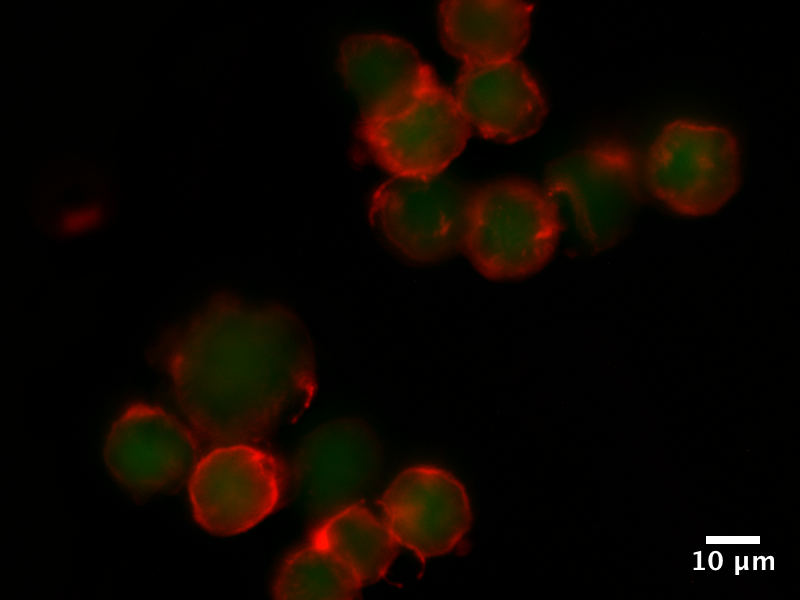
\includegraphics[width=2.3in]{FinalOverlay_Crop.png}
\caption{\textbf{Staining of non-adherent cells}. Images of LNCaP cells seeded into a device and stained immediately after seeding. EpCAM (red), GFP (green).}
\label{fig:staining}
\end{figure}

\subsection{Cell Culture}

We have used the devices presented here to culture multiple cell lines (MC3T3-E1, PC3, MCF7, and LNCaP). Initial results suggest that cell viability is not affected in any way by the process of cell concentration (data not shown). However, as with any cell-based assay, results are dependent upon many factors including the cell type and sample source. Thus, any potential bias of using this method would have to be evaluated on a case-by-case basis.

\section{Conclusions}

We have presented a method to simultaneously concentrate a suspension of cells and seed them into a microchannel that can be used for culture and the gentle application of treatment protocols. We were able leverage dimensional analysis to lower cell loss to 1.1 $\pm$ 0.6\% (avg $\pm$ SD, n = 7) via changes in device dimensions and flow rates. Data that suggests the ratio of the characteristic settling time of a cell to the estimated residence time of the cell in the collection region can be used to predict changes in cell loss with changes in device geometry and pumping parameters. Experimental data obtained under various conditions using two different device designs suggests that efficient device operation in terms of cell loss and throughput is achieved when $t_{set}/t_{res} \approx 1$. When using this method, the maximum possible cell loss is dictated by the volume used for each addition and is an important parameter to consider when attempting to reduce cell loss. Dimensional analysis suggests that the viscosity of the fluid and height of the collection region do not influence cell loss in this type of embodiment whereas the size of the cell, travel distance through the collection region, and flow rate do. The device and method increase the range of cell suspension densities that can be used with cell-based assays performed using microscale devices and provides an alternative when centrifugation is inadequate as a method for sample concentration. In this way, the technology helps to enable research on rare cell populations such as cells isolated using flow cytometry, circulating tumor cells, or primary samples from small animals. 

Specifically, we plan to use the presented microfluidic device to enable functional studies of patient CTCs. By concentrating more CTCs into fewer devices, our goal is to increase the potential for successful culture and assessment of CTCs. The ability to study CTCs on the microscale using more sensitive assays that are well-suited for limited numbers of cells could lead to less invasive monitoring of cancer treatment efficacy and a better understanding of the molecular mechanisms of cancer metastasis.

\section{Acknowledgement}

The authors would like to thank Erwin Berthier and Dr. Scott Berry for their help and suggestions with modeling and dimensional analysis of the device.  This work was supported in part by the Wallace H. Coulter Translational Research Partnership, the Department of Defense Prostate Cancer Research Program (DOD PCRP Idea Award, W81XWH-09-1-0192), and the University of Wisconsin Carbone Cancer Center.
